

\section{Sprint 2}
\subsection{Introduction}
This sprint focused on developing key features for the Patient role in MindCareAI.
It included mood tracking, journaling, group messaging, social feeds, and basic chatbot support.
Patient profiles, notifications, and user preferences were also implemented.
These features aim to enhance mental health support and user engagement.

\subsection{Sprint Backlog}
\begin{table}[H] % Changed to [H] with float package for strict placement
\centering
\begin{tabular}{|p{4.2cm}|p{7.2cm}|p{2.2cm}|}
\hline
\textbf{User Story} & \textbf{Task} & \textbf{Priorities} \\
\hline
As a user, I want my role to be assigned automatically & Implement automatic patient role assignment during registration & Low \\
\hline
As a patient, I want to manage my profile information & Create patient profile model (name, phone, blood type, gender, emergency contact) & Medium \\
\hline
As a patient, I want to upload my profile picture & Add profile picture upload functionality to profile & Low \\
\hline
As a patient, I want to track my mood daily & Implement mood logging system (1--10 scale) & High \\
\hline
As a patient, I want to log my energy levels & Add energy tracking (1--5 scale) to mood logs & High \\
\hline
As a patient, I want to link moods with activities & Add activity association to mood logs & Medium \\
\hline
As a patient, I want to view my mood trends & Display 30-day mood history and statistics & High \\
\hline
As a patient, I want to write journals & Create journaling system with content, mood, weather, activity & High \\
\hline
As a patient, I want to categorize my journal entries & Add custom categories with colors and icons & Low \\
\hline
As a patient, I want to join and leave group chats & Implement join/leave support groups & Medium \\
\hline
As a patient, I want to send group messages with media & Enable text messages (5000 chars) and media upload (images, videos, PDFs) via WebSocket & Medium \\
\hline
As a patient, I want real-time feedback in chat & Add typing indicators and read receipts (WebSocket) & Medium \\
\hline
As a patient, I want to react to and search messages & Implement message reactions and search feature & Low \\
\hline
As a moderator, I want to manage group chats & Add moderator controls (delete messages, manage users) & High \\
\hline
As a patient, I want to share posts publicly & Enable post creation with media (text, image, video) & High \\
\hline
As a patient, I want to interact on the social feed & Add likes, comments, and nested replies & Medium \\
\hline
As a patient, I want timely notifications & Implement journal, mood, message, and feed notifications (WebSocket \& email) & High \\
\hline
As a patient, I want to configure my preferences & Build display settings (dark mode, language) and notification controls & Medium \\
\hline
As a patient, I want to chat with an AI & Integrate Gemini API for basic AI chatbot responses & Medium \\
\hline
\end{tabular}
\caption{Sprint 2 Backlog -- Patient Role Features}
\end{table}


\subsubsection{Functional Analysis}
\begin{figure}[H]
    \centering
    \includegraphics[width=0.9\textwidth]{images/Chapter 4/sprint2.drawio.png}
    \caption{Sprint 2 - Use Case Diagram for Sprint 2}
    \label{fig:use_case_patient}
\end{figure}

\begin{longtable}{|p{3cm}|p{12cm}|}
\hline
\textbf{Field} & \textbf{Details} \\
\hline
Title & User Roles and Profile Management \\
\hline
Actor & Patient, System \\
\hline
Description & System automatically assigns patient role during registration and enables comprehensive profile management including personal information and profile picture \\
\hline
Condition & User must complete registration process and be authenticated \\
\hline
Output & Patient role assignment, complete profile with personal details, uploaded profile picture \\
\hline
Scenario & 1. User completes registration form with email and password credentials \newline 2. System automatically assigns patient role using Django signals during user creation \newline 3. Patient accesses their personal profile section through the secure dashboard \newline 4. Patient enters comprehensive personal information (full name, contact phone, blood type selection, gender identity, emergency contact details) \newline 5. Patient uploads profile picture with real-time preview and cropping capabilities \newline 6. System validates all input data for format and security compliance \newline 7. System securely stores profile data with encryption for sensitive fields \newline 8. Patient receives confirmation of successful profile update \\
\hline
Error handling & Registration failures, invalid profile data, profile picture upload errors, file format validation, database storage issues \\
\hline
\caption{User Roles and Profile Management Use Case}
\end{longtable}

\begin{longtable}{|p{3cm}|p{12cm}|}
\hline
\textbf{Field} & \textbf{Details} \\
\hline
Title & Mood Tracking System \\
\hline
Actor & Patient, System \\
\hline
Description & Patient logs daily mood and energy levels, associates activities, and views comprehensive mood history with trends and statistics \\
\hline
Condition & Patient must be authenticated and have active profile \\
\hline
Output & Daily mood logs, energy tracking data, activity associations, 30-day trend visualization, summary statistics \\
\hline
Scenario & 1. Patient accesses user-friendly mood tracking interface with visual mood scale indicators \newline 2. Patient rates current mood on a granular scale (1-10, where 1 is extremely negative and 10 is extremely positive) with descriptive tooltips \newline 3. Patient selects energy level from five distinct options (Very Low, Low, Moderate, High, Very High) with visual indicators \newline 4. Patient selects associated activities from a comprehensive list (Exercise, Meditation, Reading, Socializing, etc.) with multi-select capability \newline 5. Patient can add optional notes about their mood state and contextual factors \newline 6. System saves mood entry with precise timestamp and user association \newline 7. Patient views color-coded 30-day mood history with interactive data visualization \newline 8. System calculates and displays comprehensive statistics including averages, trends, patterns, and correlation between mood and activities \newline 9. Patient can export mood data for personal records or healthcare provider sharing \\
\hline
Error handling & Invalid mood/energy values, activity selection errors, data visualization issues, historical data retrieval problems \\
\hline
\caption{Mood Tracking System Use Case}
\end{longtable}

\begin{longtable}{|p{3cm}|p{12cm}|}
\hline
\textbf{Field} & \textbf{Details} \\
\hline
Title & Journaling System \\
\hline
Actor & Patient, System \\
\hline
Description & Patient creates detailed journal entries with content, mood, weather, activities and organizes them using custom categories with colors and icons \\
\hline
Condition & Patient must be logged in and have journaling access \\
\hline
Output & Journal entries with rich metadata, custom categories with visual identifiers \\
\hline
Scenario & 1. Patient opens rich journaling interface with text formatting options and templates \newline 2. Patient writes detailed journal content with support for formatting, paragraphs, and emotional expression \newline 3. Patient records current general mood state from five options (Very Negative to Very Positive) with emoji visualization \newline 4. Patient selects current weather conditions (Sunny, Cloudy, Rainy, Stormy, Snowy) to provide environmental context \newline 5. Patient tags relevant activities that influenced their mental state during the day \newline 6. Patient creates personalized categories with custom colors and icon selections for organization \newline 7. Patient assigns entry to one or multiple categories for effective journaling organization \newline 8. System automatically timestamps and associates entry with user profile \newline 9. System saves journal entry with all metadata and provides confirmation \newline 10. Patient can later search, filter, and review entries by various criteria including categories, mood, and date ranges \\
\hline
Error handling & Content validation errors, category creation failures, metadata saving issues, journal entry storage problems \\
\hline
\caption{Journaling System Use Case}
\end{longtable}

\begin{longtable}{|p{3cm}|p{12cm}|}
\hline
\textbf{Field} & \textbf{Details} \\
\hline
Title & Group Messaging Community \\
\hline
Actor & Patient, System \\
\hline
Description & Patient participates in support group messaging with real-time communication, media sharing, and moderation features using WebSocket technology \\
\hline
Condition & Patient must be authenticated and have group messaging permissions \\
\hline
Output & Real-time group messaging, media attachments, typing indicators, read receipts, message reactions, search results, moderation actions \\
\hline
Scenario & 1. Patient discovers and joins relevant support groups based on mental health topics and interests \newline 2. Patient engages in group conversations with rich text messages (supporting up to 5000 characters) delivered instantly via WebSocket technology \newline 3. Patient receives real-time notifications when new messages arrive in any joined groups \newline 4. Patient uploads diverse media attachments (images for visual expression, videos for deeper sharing, PDFs for informational resources) with preview capabilities \newline 5. System displays real-time typing indicators showing which group members are composing messages \newline 6. System tracks and displays message read receipts to confirm message delivery and viewing \newline 7. Patient uses message reactions (emoji responses) for quick emotional feedback without typing \newline 8. Patient employs advanced search functionality to find specific content in conversation history \newline 9. Moderators have enhanced permissions to remove inappropriate content, mute disruptive users, and maintain supportive community standards \newline 10. System maintains message history for continuity of support and reference \newline 11. Patient can gracefully exit groups when needed while preserving past contributions \\
\hline
Error handling & WebSocket connection failures, media upload errors, message validation issues, moderation action failures, search functionality problems \\
\hline
\caption{Group Messaging Community Use Case}
\end{longtable}

\begin{longtable}{|p{3cm}|p{12cm}|}
\hline
\textbf{Field} & \textbf{Details} \\
\hline
Title & Social Feeds \\
\hline
Actor & Patient, System \\
\hline
Description & Patient creates and shares posts with media content and engages with community through likes, comments, and nested comment discussions \\
\hline
Condition & Patient must be authenticated and have social feed access \\
\hline
Output & Public posts with media content, engagement metrics (likes), comment threads with nested replies \\
\hline
Scenario & 1. Patient creates new post with formatted text and selectable post topics for better categorization \newline 2. Patient enhances posts with multi-media content (images, videos) with automatic format optimization \newline 3. Patient adds relevant tags to increase post discoverability within the community \newline 4. Patient publishes post to the social feed with privacy level selection options \newline 5. Patient browses personalized community posts with topic filtering capabilities \newline 6. Patient expresses appreciation through likes with immediate visual feedback \newline 7. Patient engages in meaningful discussions through detailed comments on posts \newline 8. Patient participates in threaded conversations through nested replies (supporting multiple levels) \newline 9. System tracks all engagement metrics for content relevance algorithms \newline 10. Users receive real-time notifications when others engage with their content \newline 11. System automatically detects and flags potentially inappropriate content for review \\
\hline
Error handling & Post creation failures, media upload errors, engagement tracking issues, nested comment depth limitations, content moderation problems \\
\hline
\caption{Social Feeds Use Case}
\end{longtable}

\begin{longtable}{|p{3cm}|p{12cm}|}
\hline
\textbf{Field} & \textbf{Details} \\
\hline
Title & Notification System \\
\hline
Actor & Patient, System \\
\hline
Description & System delivers real-time notifications for journal activities, messaging alerts, mood tracking reminders, and feed engagement using WebSocket technology \\
\hline
Condition & Patient must be authenticated and have notification permissions enabled \\
\hline
Output & Real-time notifications for journal confirmations, messaging alerts, mood reminders, feed engagement notifications \\
\hline
Scenario & 1. System continuously monitors user-related activities across all platform features requiring notification alerts \newline 2. System generates and sends journal creation confirmations with entry summary for user verification \newline 3. System delivers instant messaging alerts for new messages with sender preview through WebSocket connections \newline 4. System shows real-time typing indicators when group members are composing messages \newline 5. System sends personalized mood tracking reminders based on user habit patterns and preferences \newline 6. System generates notifications about social feed engagement (likes, comments, replies) with engagement preview \newline 7. Patient receives prioritized notifications in real-time with visual and optional sound indicators \newline 8. System delivers alternative notification delivery through email for important offline updates \newline 9. Notifications remain in queue until acknowledged or marked as read by the patient \newline 10. System applies user preference filters before delivering notifications to respect user settings \\
\hline
Error handling & WebSocket delivery failures, notification timing issues, permission errors, notification queue overload \\
\hline
\caption{Notification System Use Case}
\end{longtable}

\begin{longtable}{|p{3cm}|p{12cm}|}
\hline
\textbf{Field} & \textbf{Details} \\
\hline
Title & User Preferences Management \\
\hline
Actor & Patient, System \\
\hline
Description & Patient customizes application experience through display settings and notification controls with selective notification management \\
\hline
Condition & Patient must be authenticated and have access to preferences \\
\hline
Output & Customized display settings, configured notification preferences, selective notification controls \\
\hline
Scenario & 1. Patient accesses comprehensive user preferences interface through profile settings \newline 2. Patient configures visual display preferences including dark/light mode with preview functionality \newline 3. Patient selects preferred language from supported options with immediate interface translation \newline 4. Patient customizes notification delivery channels (toggles between email, in-app, or both) \newline 5. Patient configures notification frequency settings to prevent overwhelming alerts \newline 6. Patient granularly enables/disables specific notification types by category (journaling, mood, messaging, feeds) \newline 7. Patient sets quiet hours during which non-critical notifications are suppressed \newline 8. System validates and applies all preference changes in real-time \newline 9. System securely stores preference settings in user profile \newline 10. System consistently applies saved preferences across all sessions and devices \newline 11. Patient can reset preferences to default values if needed \\
\hline
Error handling & Preference saving failures, display setting application errors, notification control conflicts, session persistence issues \\
\hline
\caption{User Preferences Management Use Case}
\end{longtable}

\begin{longtable}{|p{3cm}|p{12cm}|}
\hline
\textbf{Field} & \textbf{Details} \\
\hline
Title & Basic AI Chatbot \\
\hline
Actor & Patient, System \\
\hline
Description & Patient interacts with AI-powered chatbot integrated with Gemini API for simple conversational responses and basic user interaction support \\
\hline
Condition & Patient must be authenticated and have chatbot access enabled \\
\hline
Output & AI-generated conversational responses, basic interaction support, conversation history \\
\hline
Scenario & 1. Patient accesses AI chatbot interface \newline 2. Patient sends message or question to chatbot \newline 3. System processes request through Gemini API integration \newline 4. System generates simple conversational response \newline 5. Patient continues basic user interaction \newline 6. System maintains conversation context \\
\hline
Error handling & Gemini API connection failures, response generation timeouts, inappropriate content filtering, conversation context errors \\
\hline
\caption{Basic AI Chatbot Use Case}
\end{longtable}
\newpage

\subsection{Database Design}

This subsection presents the database schema used in the system. The design ensures data integrity, scalability, and normalization.
 
\vfill
\begin{figure}[H]
    \centering
    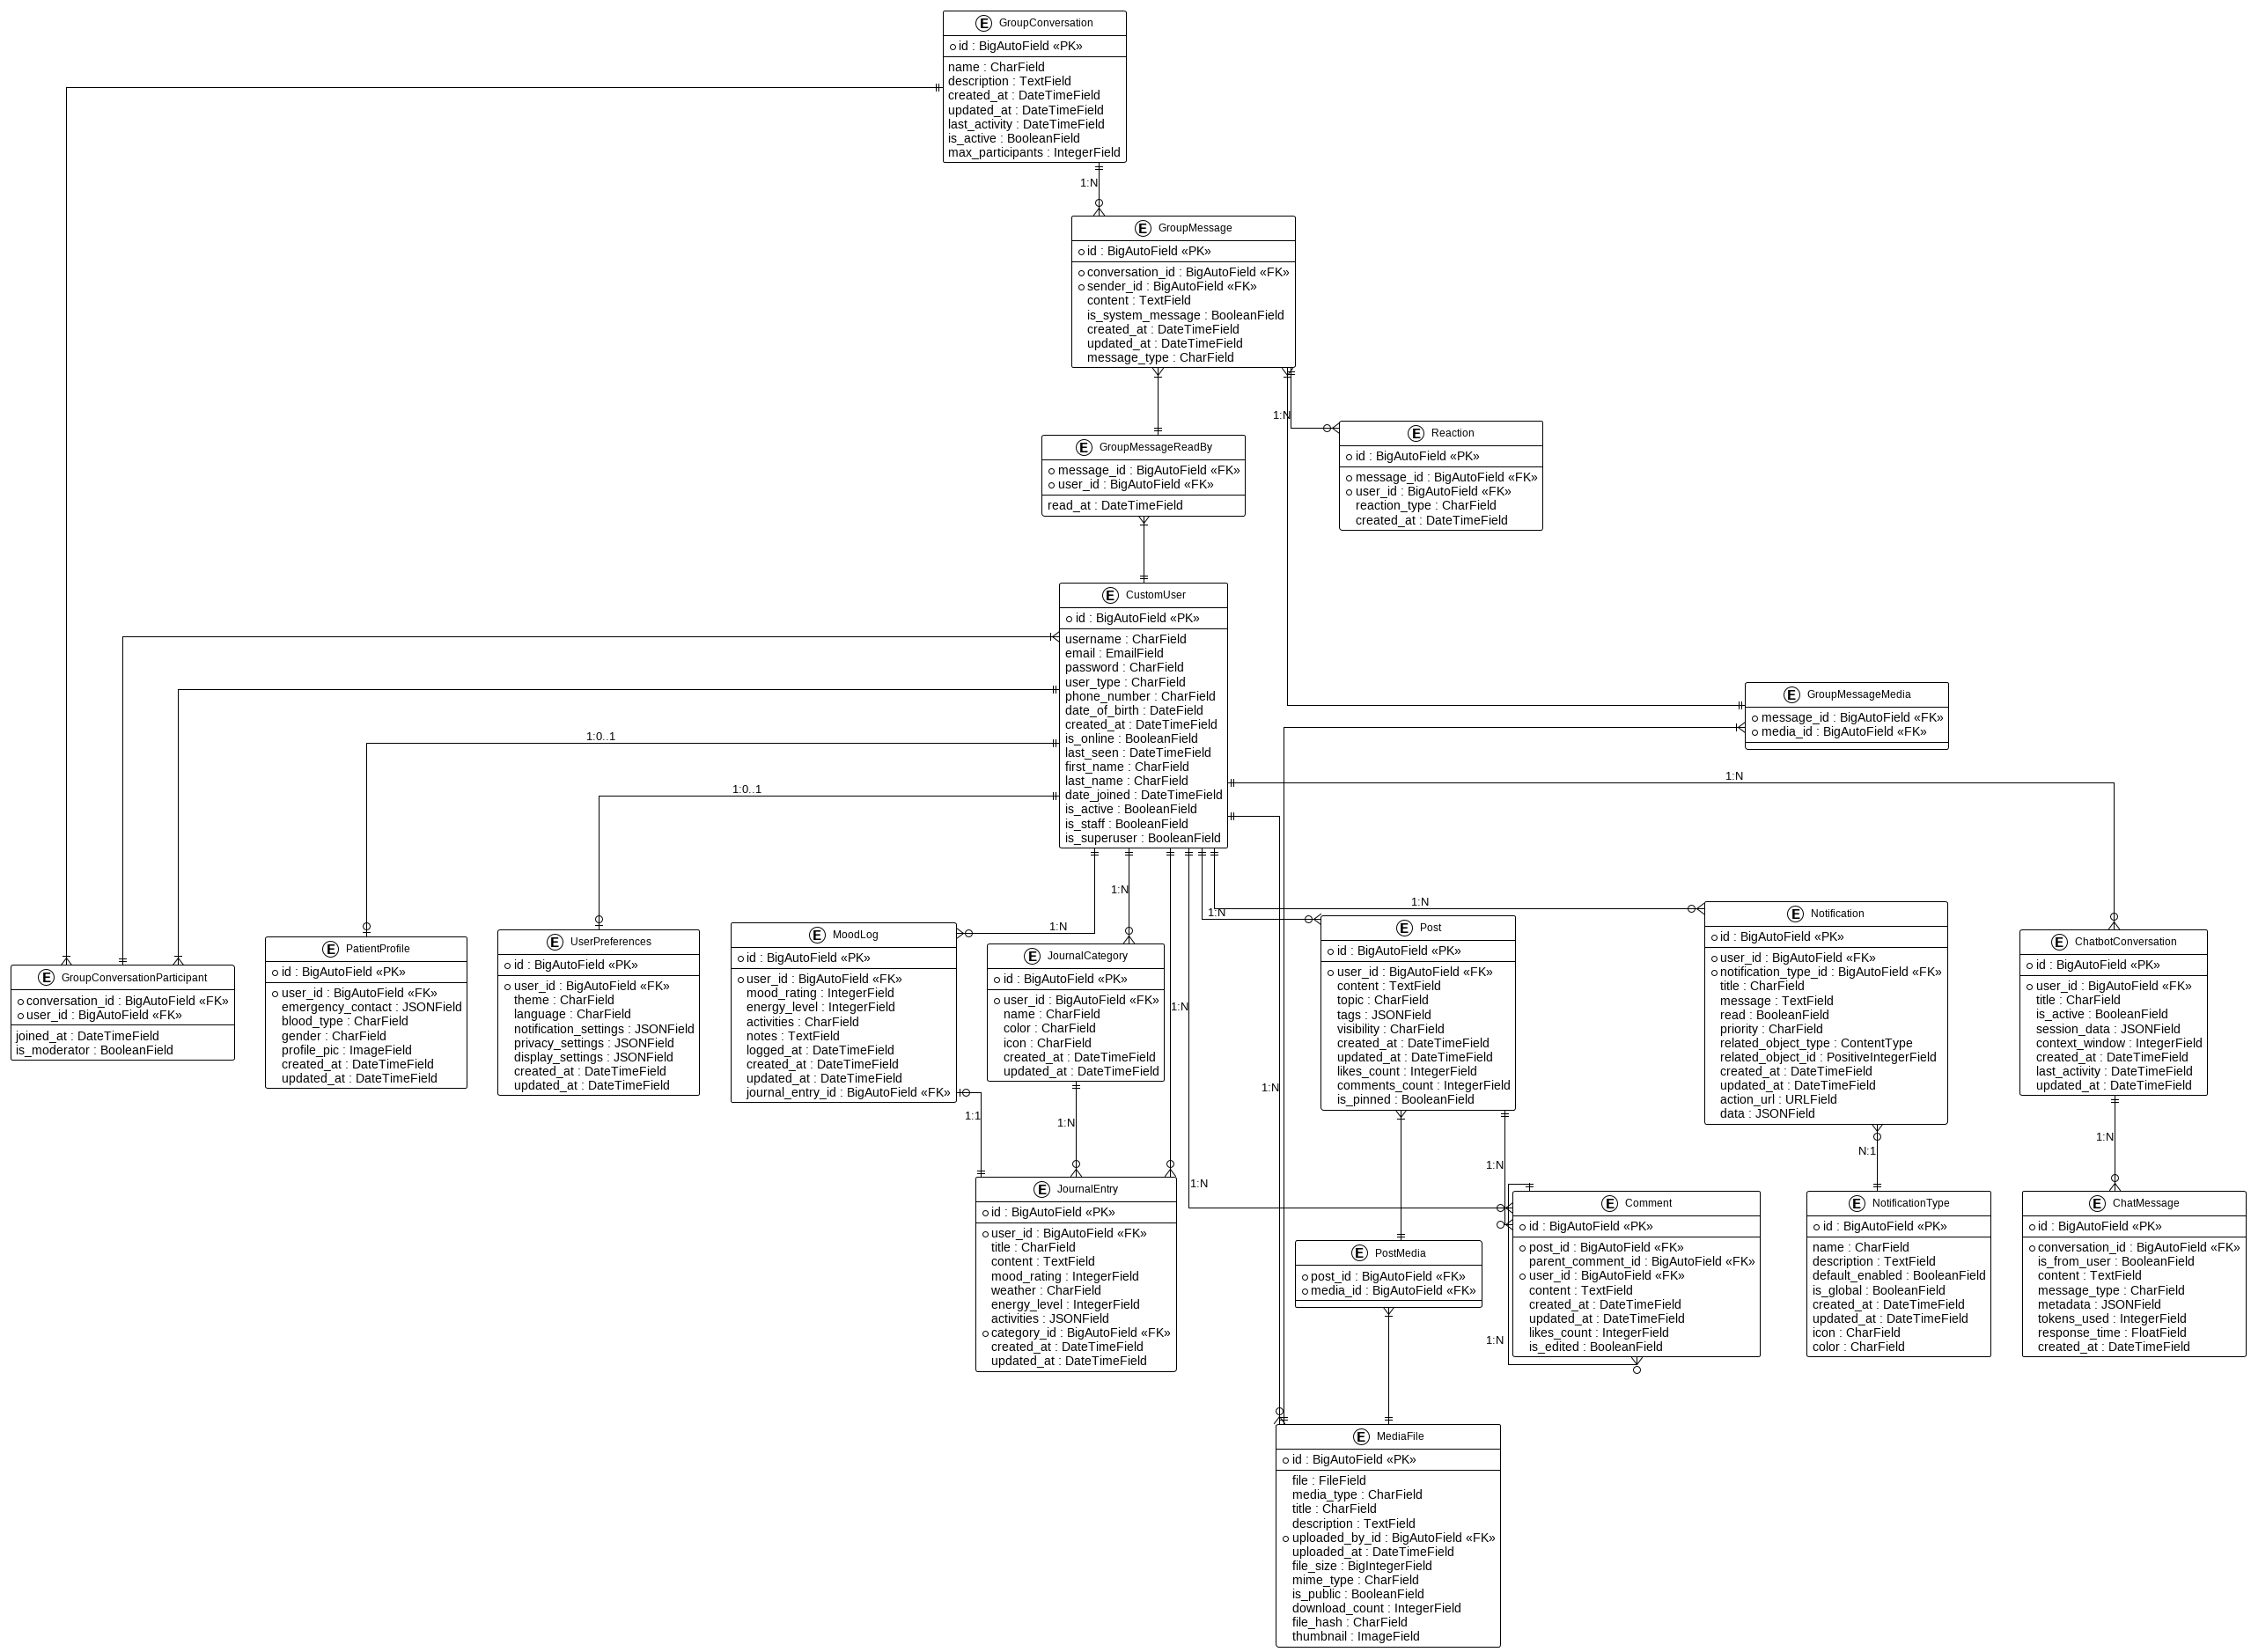
\includegraphics[width=0.95\textheight, height=0.95\textwidth, angle=90]{images/Chapter 4/Sprint2_ERD.png}
    \caption{Database Design Diagram}
    \label{fig:database-design}
\end{figure}



\vfill
\newpage

\subsection{Software Design}

This section provides a structural and behavioral view of the software system using UML diagrams.

\paragraph{Class Diagram}

The class diagram outlines the static structure of the system, detailing the classes, attributes, methods, and relationships.

\begin{figure}[H]
    \centering
    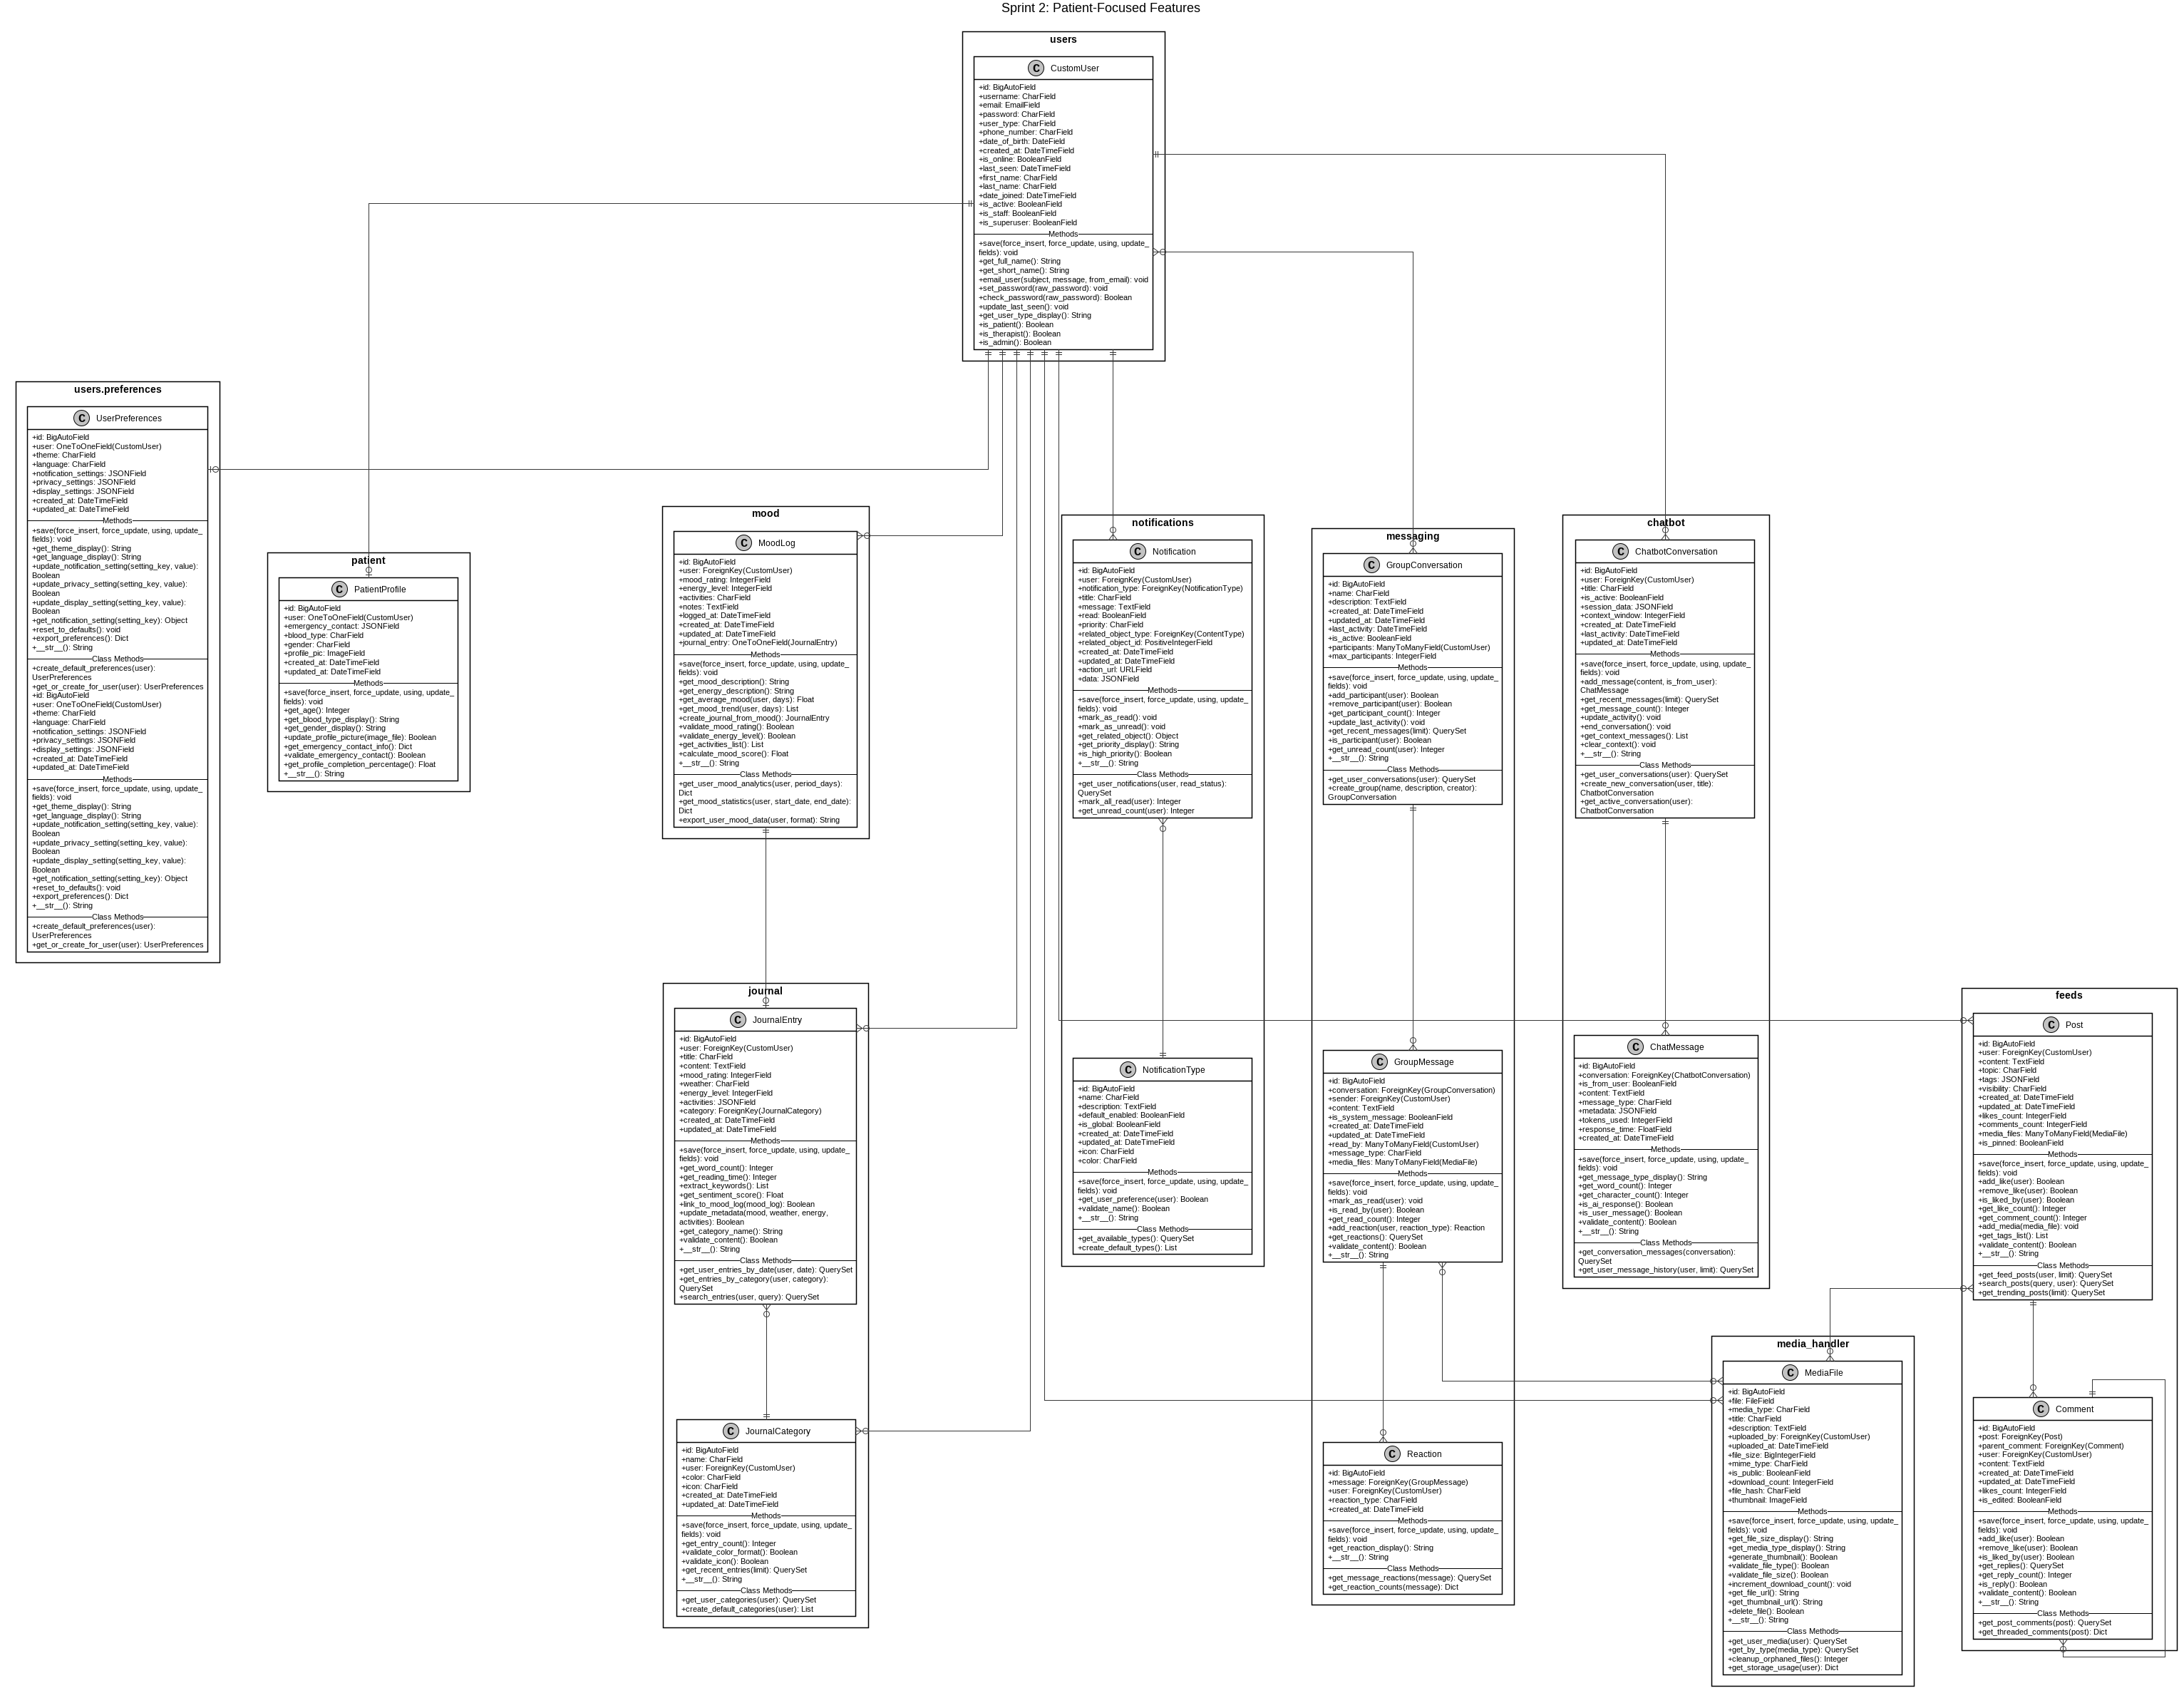
\includegraphics[width=1\textheight, height=0.95\textwidth, angle=90]{images/Chapter 4/sprint2_class_diagram.png}
    \caption{Class Diagram of the System}
    \label{fig:class-diagram}
\end{figure}

\paragraph{Sequence Diagrams}

The following sequence diagrams illustrate the dynamic behavior of each major system component, focusing on object interactions over time for each Django application in Sprint 2.

\begin{figure}[H]
    \centering
    \includegraphics[width=0.75\textwidth]{images/Chapter 4/sprint2/Auth_Sequence_Diagram.png}
    \caption{Authentication \& Role Assignment Sequence Diagram}
    \label{fig:auth-sequence-diagram}
\end{figure}

\begin{figure}[H]
    \centering
    \includegraphics[width=0.75\textwidth]{images/Chapter 4/sprint2/Patient_Sequence_Diagram.png}
    \caption{Patient Profile Management Sequence Diagram}
    \label{fig:patient-sequence-diagram}
\end{figure}

\begin{figure}[H]
    \centering
    \includegraphics[width=0.65\textwidth]{images/Chapter 4/sprint2/Mood_Sequence_Diagram.png}
    \caption{Mood Tracking }
    \label{fig:mood-sequence-diagram}
\end{figure}

\begin{figure}[H]
    \centering
    \includegraphics[width=0.45\textwidth]{images/Chapter 4/sprint2/Messaging_Sequence_Diagram.png}
    \caption{Group Messaging System Sequence Diagram}
    \label{fig:messaging-sequence-diagram}
\end{figure}

\begin{figure}[H]
    \centering
    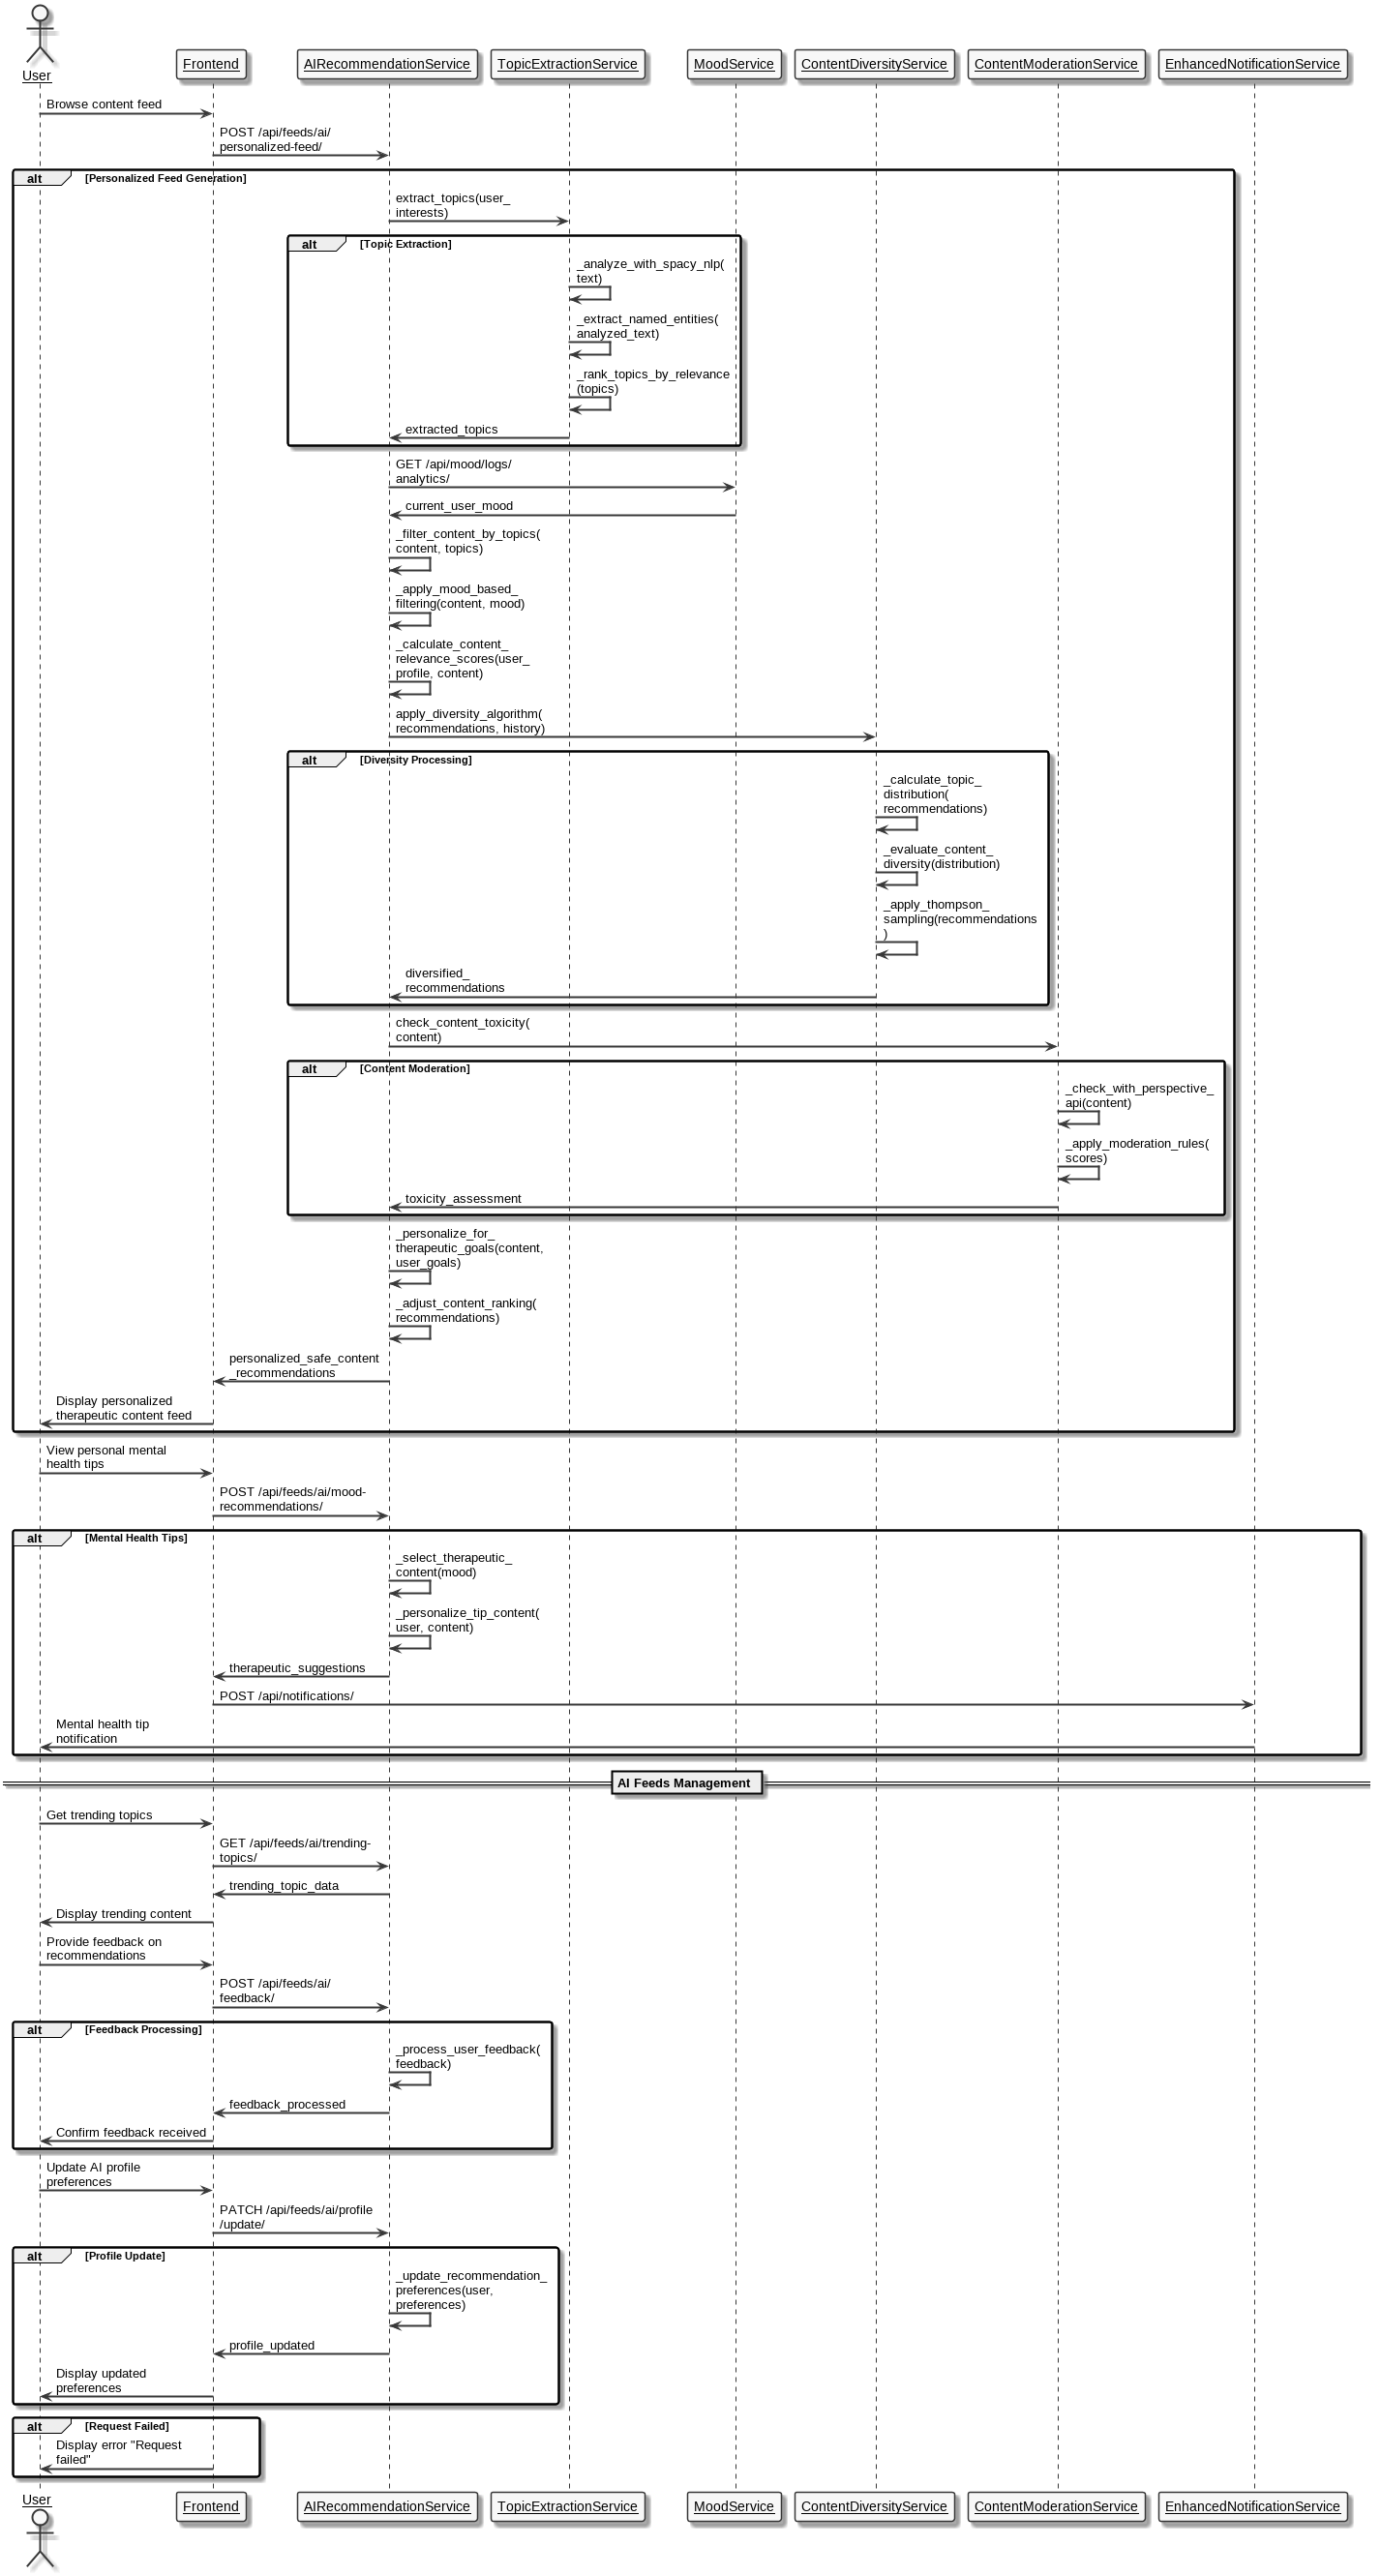
\includegraphics[width=0.70\textwidth]{images/Chapter 4/sprint2/Feeds_Sequence_Diagram.png}
    \caption{Social Feed System Sequence Diagram}
    \label{fig:feeds-sequence-diagram}
\end{figure}

\begin{figure}[H]
    \centering
    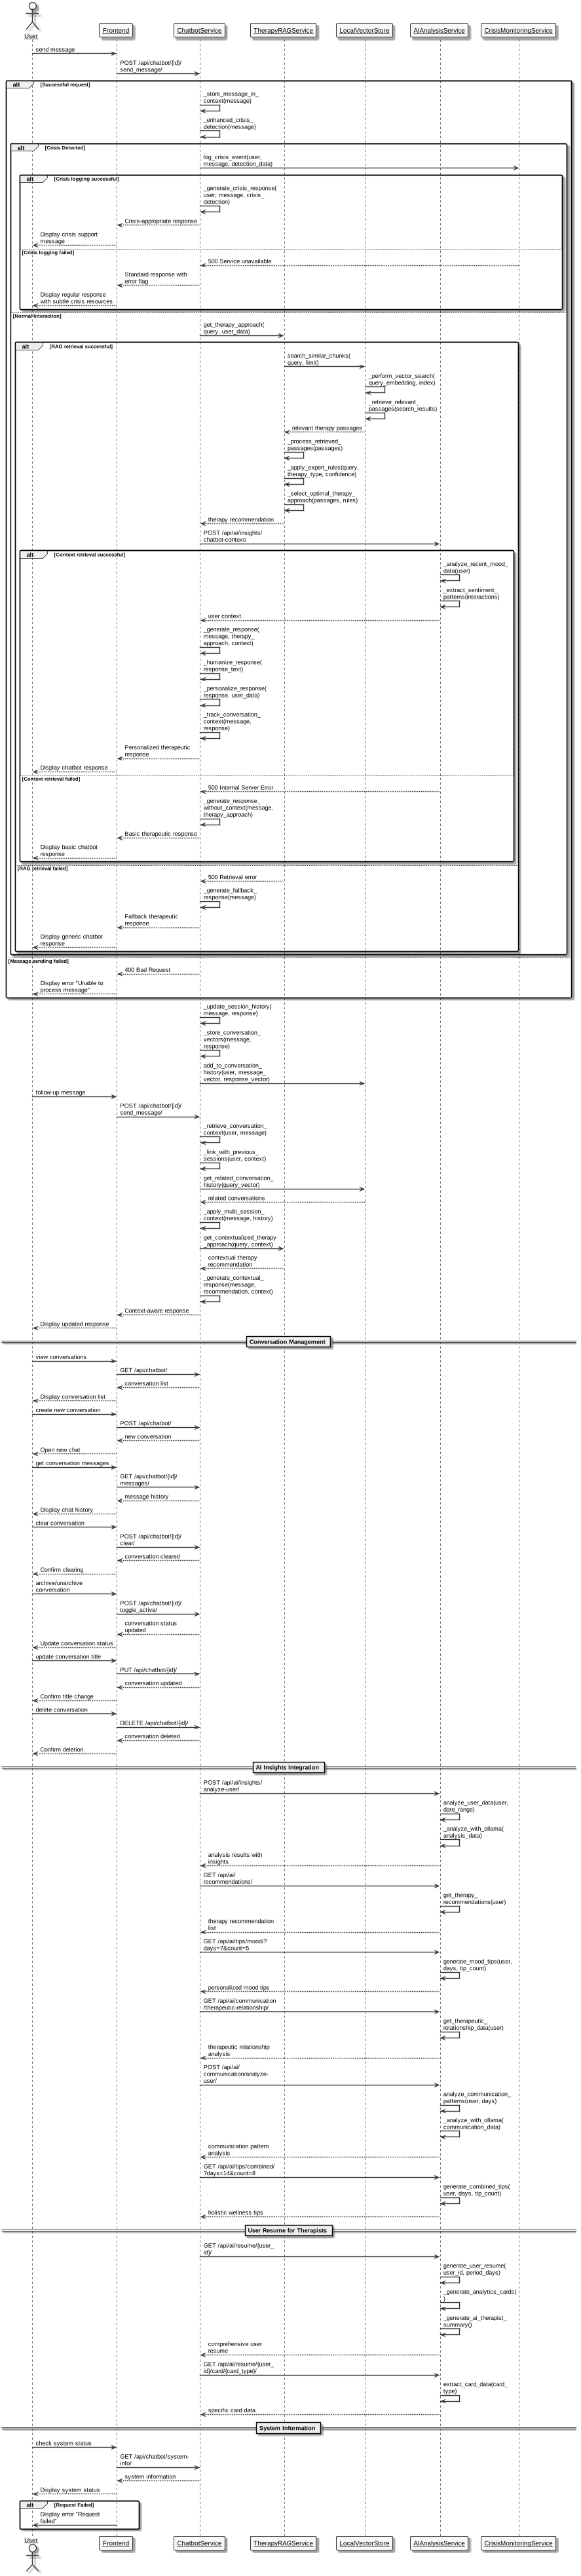
\includegraphics[width=0.70\textwidth]{images/Chapter 4/sprint2/Chatbot_Sequence_Diagram.png}
    \caption{AI Chatbot System Sequence Diagram}
    \label{fig:chatbot-sequence-diagram}
\end{figure}
\begin{figure}[H]
    \centering
    \includegraphics[width=0.55\textwidth]{images/Chapter 4/sprint2/Journal_Sequence_Diagram.png}
    \caption{journal Sequence Diagram}
    \label{fig:journaling-sequence-diagram}
\end{figure}